\documentclass{article}
\usepackage{fontspec}
\usepackage{polyglossia}
\setdefaultlanguage{french}
\usepackage[a4paper,margin=2.5cm]{geometry}

\usepackage{amsmath}
\usepackage{amssymb}
\usepackage{array}
\usepackage{auto-pst-pdf}
\usepackage{booktabs}
\usepackage{cite}
\usepackage{graphicx}
\usepackage{lmodern}
\usepackage{marvosym}
\usepackage{mathrsfs}
\usepackage{minted}
\usepackage{multicol}
\usepackage{multirow}
\usepackage{paralist}
\usepackage{schemabloc}
\usepackage{siunitx}
\usepackage{soul}
\usepackage{tikz}
\usepackage[european,cuteinductors,siunitx]{circuitikz}
\usepackage{url,hyperref}
\usepackage{verbatim}
\usepackage{xunicode,xltxtra}

\title{
\includegraphics{../../../images/inp-enseeiht} \\ ~ \\ ~ \\ ~ \\ ~ \\ Salle Blanche}
\author{François Pierron \& Guilhem Saurel}
\date{\oldstylenums{24 janvier 2014}}

\begin{document}

\begin{titlepage}
    \setcounter{page}{0}
    \maketitle
    \vfill
    \tableofcontents
    \thispagestyle{empty}
\end{titlepage}

\section*{Introduction}

Ceci est le rapport d’une semaine passée en salle blanche à l’AIME lors de laquelle nous avons fabriqué, étape par étape, un wafer de silicium, de la croissance du premier oxyde à la mise dans un boitier de l’une des puces et à son test.

\section{Étape préliminaire}

Nous disposons d’un wafer de 2” de diamètre et d’épaisseur que nous mesurons de 304µm.

C’est un substrat de type P, d’orientation 100, nous mesurons sa résistivité par une mesure à 4 pointes pour en évaluer le dopage intrinsèque.

~

Le test à 4 pointes en ligne nous donne une valeur de $17.5 \Omega$, soit une résistivité de $17.5 \Omega$ cm, ce qui donne, après lecture sur l'abaque, un dopage intrinsèque de $8\cdot10^{14}$ cm$^{-3}$ environ. C’est beaucoup plus faible que ce qui était annoncé par le fabricant ($\simeq 1\cdot10^{16}$) mais les mesures des autres groupes confirment ce résultat.

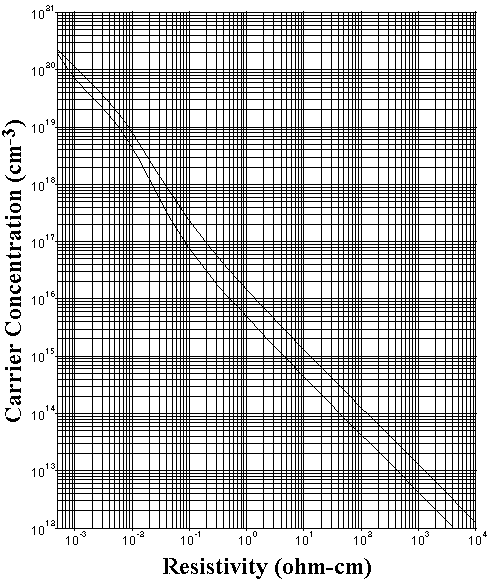
\includegraphics[width=\linewidth-2cm]{calc_res.png}

\section{Oxydation de masquage}

Nous commençons par nettoyer le wafer puis l’enfournons pour réaliser la première oxydation.

Nous utilisons le premier témoin pour mesurer l’épaisseur de cet oxyde : nous protégeons une partie du témoin avec un adhésif et nous attaquons l’autre partie au buffer HF, nous en profitons pour relever le temps nécessaire pour attaquer complètement l’oxyde : 5’55”.

~

Nous enlevons l’adhésif et mesurons au profilomètre la hauteur de la chute entre la partie oxydée et la partie sans oxyde : 4932 A°.
Ce qui correspond au résultat attendu avec les abaques : 40 minutes à 1100 C° donne environ 5000 A°.

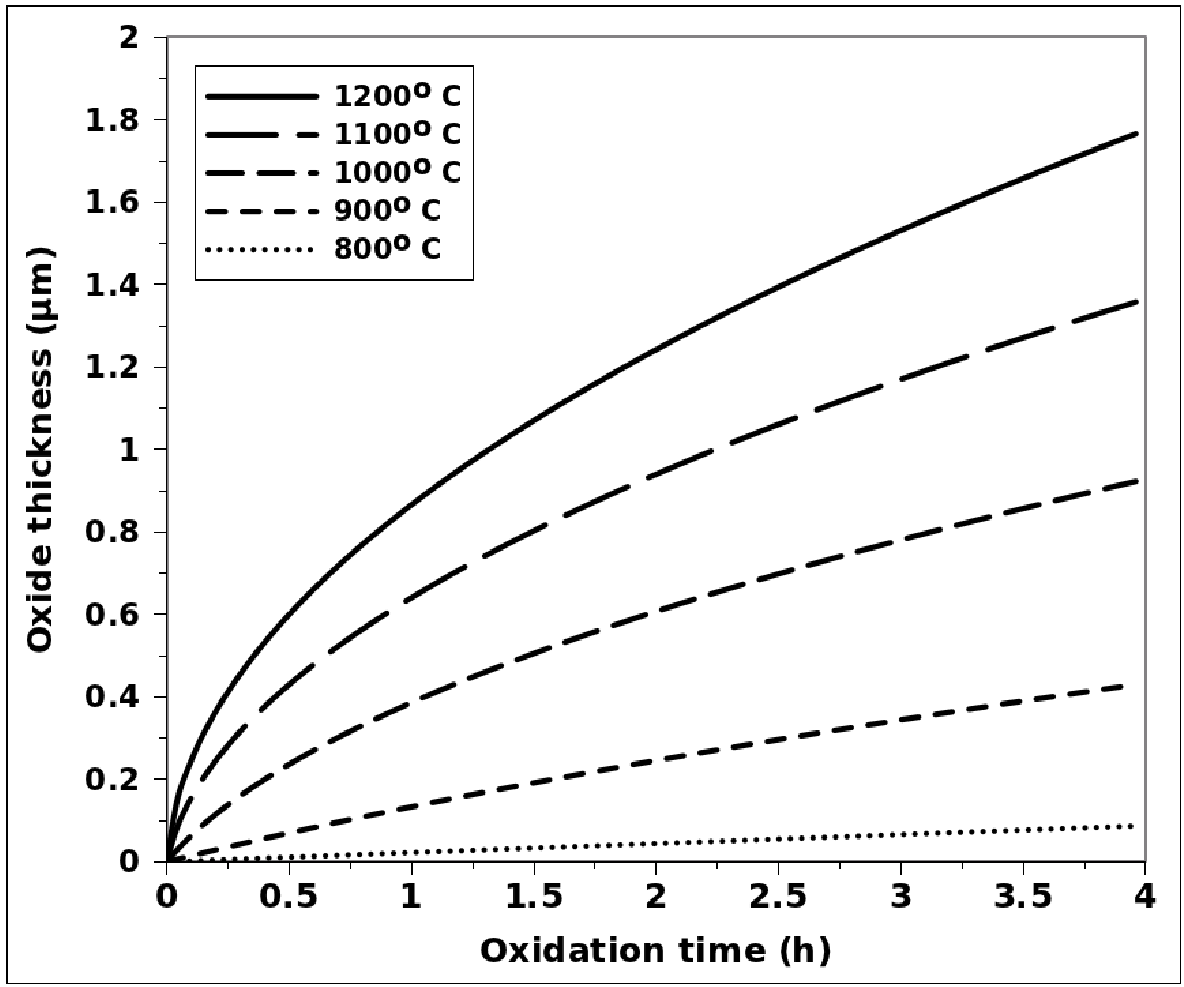
\includegraphics[width=\linewidth]{img160.png}

\section{Photolithographie: ouverture des transistors}

Nous réalisons la première photolithographie et gravons avec le temps obtenu précédemment : 5’55”.

\section{Oxydation de grille}

Après un nettoyage le wafer subit une oxydation sèche pour réaliser l’oxyde de grille. Il faut une faible épaisseur, et c’est pour ça que l’oxydation sèche est préférée car elle est beaucoup plus lente.

En utilisant la même méthode qu’au 1, nous mesurons l’épaisseur d’oxyde:

% LOIC

au profilomètre : 77.7 nm

à l’ellipsomètre : 74.02 nm

Ces valeurs sont supérieures à celles que l’on pouvait attendre : 20 minutes à 1100 C° donnant plutôt 45 nm.

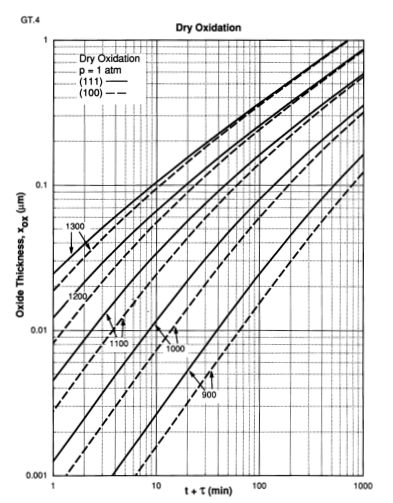
\includegraphics[width=\linewidth]{gt4.png}

\section{Dépôt de polysilicium}

La grille en polysilicium est réalisée dans un réacteur LPCVD.
Nous utilisons un témoin pour mesurer le temps d’attaque nécessaire pour enlever tout le poly déposé puis nous mesurons son épaisseur au profilomètre : 330 nm ainsi que sa résistivité avec le test sous pointes :$ 1.4 \Omega$ cm

\section{Gravure du polysilicium}

Afin de fabriquer les Gates des transistors MOS, il faut ouvrir la source et le drain, cela est fait avec une nouvelle photolithographie, la gravure se fait grâce au temps relevé à l’étape précédente.
Pour aligner les masques ensembles, nous utilisons des mires, ici, les 3 mires correspondent à ce qui a été réalisé lors de l’ouverture du transistor (étape précédente), et le carré dans la première correspond au masquage de cette étape, bien au centre de la mire, et a créé 2 nouvelles mires pour les étapes suivantes.

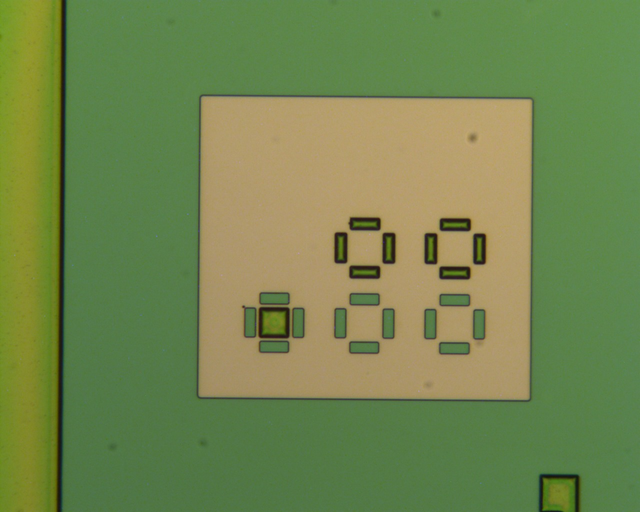
\includegraphics[width=\linewidth]{mire_poly.png}

\section{Diffusion source et drain}

Nous réalisons maintenant la diffusion, c’est à dire le dopage des drains et des sources des transistors. Cette diffusion se fait en 2 étapes : un prédépot dans un four, puis une redistribution dans un autre four pour permettre aux atomes de phosphore de se répartir un peu mieux.

Sur un wafer témoin, à l’aide d’un rouleau de rodage et de pâte diamantée, nous observons la profondeur de jonction au microscope et obtenons 1.15 µm.

Nous mesurons aussi la résistivité du silicium dopé : $1.14 \Omega$ cm ce qui donne un dopage à $4\cdot10^{15}$~cm~$^{-3}$.

\section{Dépôt de SiO2 LTO}

Maintenant que les transistors sont réalisés, il faut prévoir ce qu’il faut pour les relier entre-eux, pour cela, nous commençons par déposer une couche de SiO2 isolant sur tout le wafer, de manière à pouvoir ensuite faire des pistes de métal sans tout court-circuiter par la suite.

Nous déposons donc du SiO2 dans un four LPCVD.

Nous mesurons l’épaisseur déposée à l’ellipsomètre : 301 nm et en profitons pour relever le temps d’attaque.

\section{Ouverture des contacts}

Nous réalisons ensuite la 3eme photolithographie pour réaliser les contacts: il faut que le métal puisse accéder aux transistors là ou c’est nécessaire.

Nous utilisons les mires des étapes précédentes pour s'aligner, tout en rajoutant une mire supplémentaire pour la dernière étape.

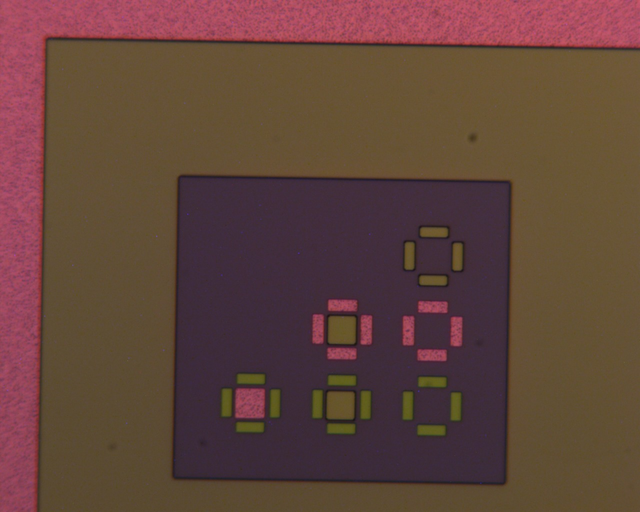
\includegraphics[width=\linewidth]{mire_contacts.png}

La gravure se fait grâce au temps trouvé à l’étape précédente.

\section{Métallisation}

Afin de réaliser les pistes pour relier les transistors entre-eux, nous déposons une couche d'aluminium sur le Sio2 isolant déposé précédemment, l’alluminium ira aussi se déposé au fond des trous réalisés dans le SiO2 pour les contacts avec les grilles, les drains et les sources des transistors.

Sur un témoin, on mesure un dépot de 272,8 nm.

\section{Gravure du métal}

On réalise la dernière photolithographie pour dessiner les pistes dans le métal.

On s’aligne grâce aux 3 mires correspondantes aux 3 étapes de gravure précédentes.

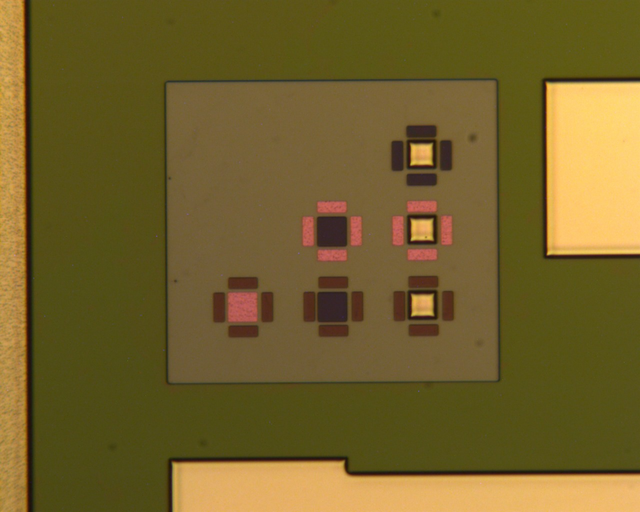
\includegraphics[width=\linewidth]{mire_alu_grave.png}

Une fois la gravure de l’aluminium faite, nous décapons l’arrière du wafer de manière à avoir accès a la polarisation du substrat.

Une fois cela fait, un dernier recuit est effectué pour stabiliser le métal.

\section*{Conclusion}

Après une semaine à fabriquer et à caractériser ces puces, nous avons été vraiment heureux de voir qu’elles marchaient correctement.

~

Cette semaine était relativement intense et nous n’avions pas droit à l’erreur. Cela a été pour nous une excellente expérience où nous avons énormément appris tout en appréciant ce que nous avons fait.

~

Nous sommes donc particulièrement tristes d’avoir certains problèmes entre le passage dans cette salle et la rédaction du présent rapport qui nous ont conduit à ne pas pouvoir en faire autant que nous aurions voulu.

\newpage
\section*{Galerie}
%\begin{multicols}{2}
    \begin{centering}


    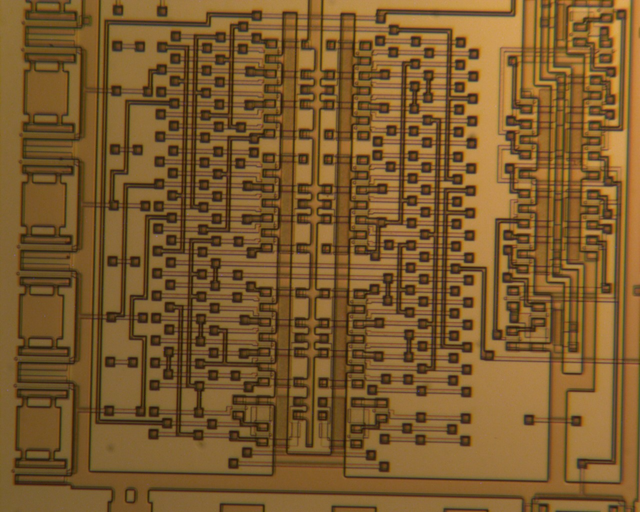
\includegraphics[width=\linewidth-2cm]{circuit_alu.png}

    Un circuit réalisé

    ~

    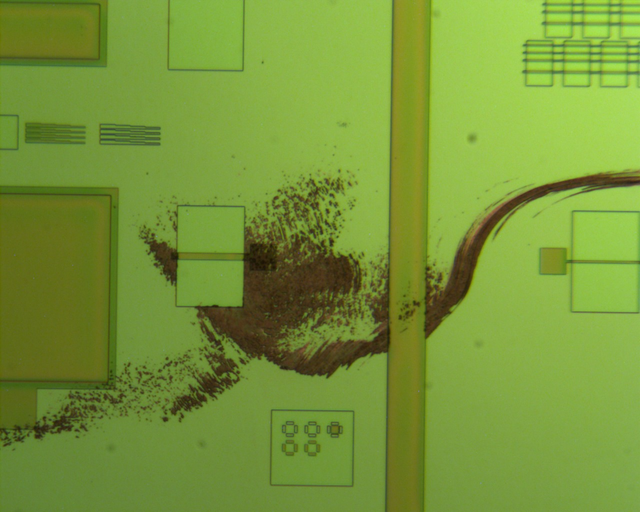
\includegraphics[width=\linewidth-2cm]{coup_de_pince.png}

    Une belle égratignure

    ~

    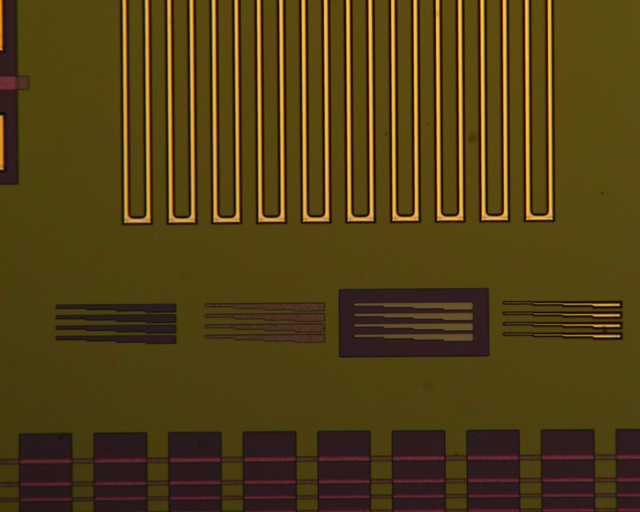
\includegraphics[width=\linewidth-2cm]{peignes.png}

    les peignes pour vérifier les gravures

    ~

    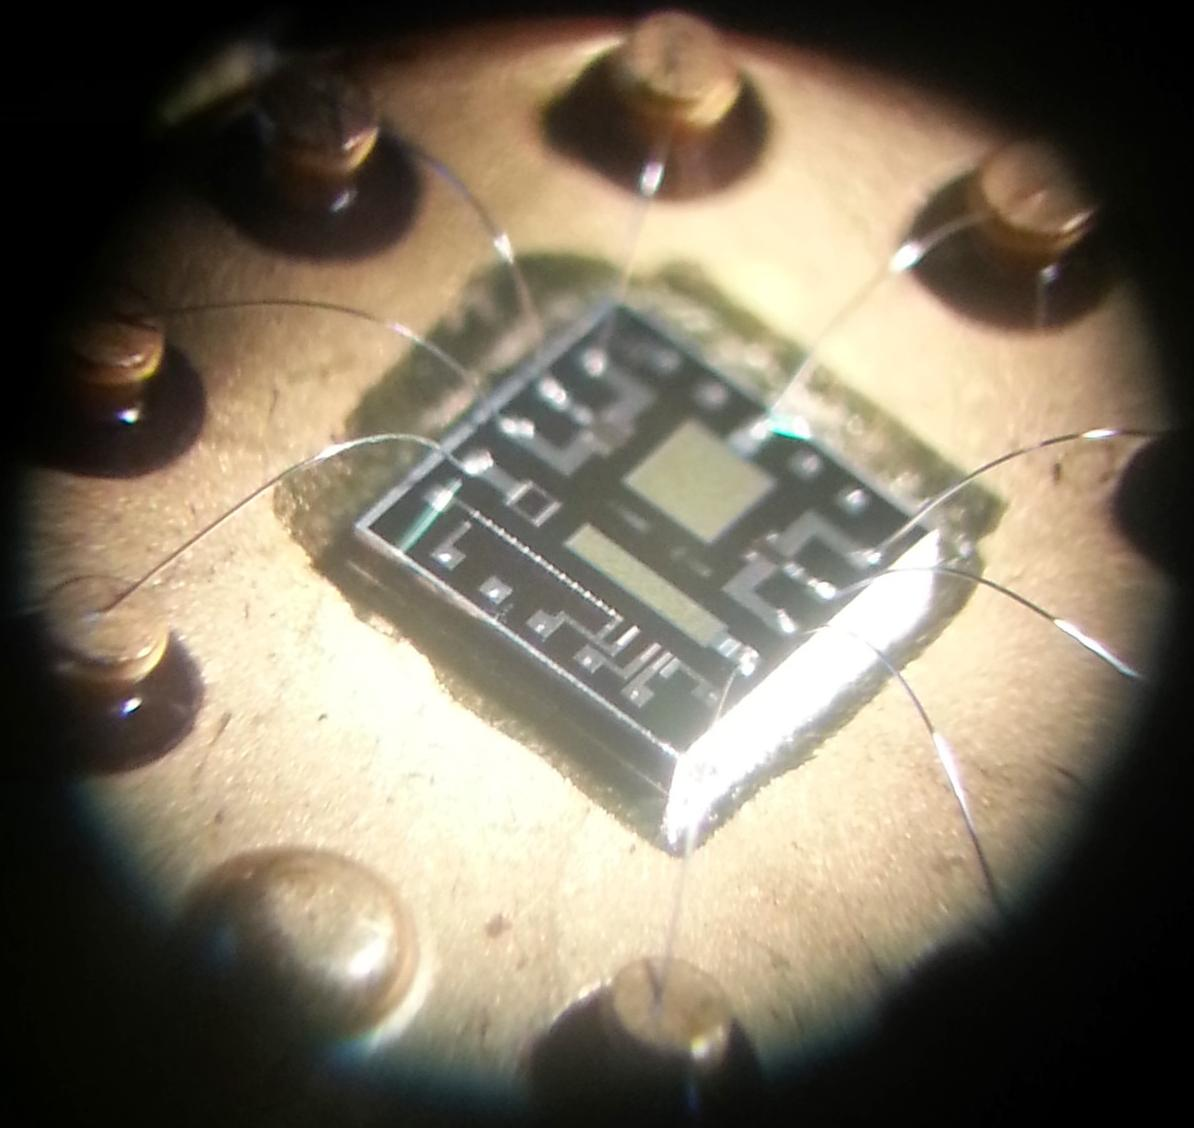
\includegraphics[width=\linewidth-4cm]{photo.jpg}

    Une puce dans son boitier

\end{centering}
%\end{multicols}

\end{document}
